\section{Lepton couplings for simplified %Uli: dark matter 
DM models}
\label{sec:models}

%The model choices made for the early Run-2 LHC searches by the ATLAS/CMS DM Forum~\cite{Abercrombie:2015wmb} assume that the DM particle is a Dirac fermion~$\chi$.
%The new particle mediating the interaction (the ``mediator") is either a vector, an axial vector, a scalar or a pseudo-scalar, and it can be exchanged either in the $s$-channel or in the $t$-channel. In the limit of large $\mmed$, these (and all) models converge to a universal set of operators in an effective field theory (EFT)
%\cite{Beltran:2010ww,Goodman:2010yf,Bai:2010hh,Goodman:2010ku,Rajaraman:2011wf,Fox:2011pm,Bell:2015sza}.

% KH, reorganized the above


The simplified models recommended by the ATLAS/CMS DMF~\cite{Abercrombie:2015wmb} assume that DM is a Dirac fermion~$\chi$ and there is an additional heavy particle mediating the SM-DM interaction (the ``mediator"). In the most basic set of these models, the mediator is a vector, an axial-vector, a scalar or a pseudo-scalar boson. So far, ATLAS and CMS have focused on the subset of the models where the mediator is exchanged in the $s$-channel. These models contain four free parameters. In the vector and axial-vector models, the parameters are the DM mass~$\mDM$, the mediator mass~$\mmed$, the coupling~$\gDM$ of a mediator-DM-DM vertex, and the coupling~$\gq$ universal to all mediator-quark-quark vertices. In the scalar and pseudo-scalar models, a quark-mass-dependent Yukawa factor scales the coupling of the mediator-quark-quark vertices to avoid violating flavor constraints. These four quantities parameterize the production rate of the mediator in proton-proton collisions, its quark and DM decay rates, and the kinematic distributions of signal events.

Complete models of DM can contain mediators that may have (or require for consistency) couplings to other SM particles that are not found in the simplified models above. Such couplings would introduce additional decay modes of the mediator at the LHC as well as further DM annihilation channels in the relic density calculation. In this section, we discuss why and how to add lepton couplings to the vector and axial-vector simplified models, provide formulas for the total decay width of the mediators, and discuss the implementations of these models that are currently available. We then propose four benchmark scenarios for comparing di-jet, di-lepton, and mono-$X$ searches, based on rough estimates of the sensitivity of these searches with $30 \, {\rm fb}^{-1}$ of LHC data. We also comment on the interference between the mediator di-lepton process and the Drell-Yan backgrounds to di-lepton searches. 

%\footnote{An orthogonal set of models describe $t$-channel exchange \cite{Chang:2013oia,An:2013xka,Bai:2013iqa,DiFranzo:2013vra}. This class of simplified DM models is left for future iterations and will thus not be discussed in the following. \textcolor{red}{KH -- I think we will include this in the paper ...}
%\textcolor{cerulean}{CD -- yes, but I've removed for now since this will go to the dilepton analysers}} 

%CD: we have to discuss whether the following is included in this document
%, and mixing with the Higgs boson in scalar-mediated simplified models.  This recommendedation also briefly addresses t-channel (refs?) and two-Higgs doublet models (2HDM, refs?), which should be studied in the near term so that LHC searches can be interpreted in this expanded class of models after Moriond 2017.

\subsection{Charged lepton couplings in vector and axial-vector simplified models}
\label{sub:vecAxial}

Simplified models are designed to capture the coarse details of collider phenomenology found in complete, rigorously-derived theories of new physics, without the attendant complexity of the full theory, particularly physics at energy scales that cannot be accessed at the collider. The ATLAS/CMS DMF focused on the phenomenology of MET signatures at the LHC. In the simplified DMF models involving spin-1 mediators,\footnote{In this document, we will focus on the case of spin-1 mediators, and postpone the discussion of scalar and pseudo-scalar mediators to future work.} quark couplings provide $pp$ collider production, and DM couplings provide the decays to DM. These two couplings set a ``minimal width" for the spin-1 resonance. 
%The effects of optional couplings to other SM particles were encoded via the additional width these couplings would generate. {\bf [Uli: I think that this has not been done in the DMF report, at least not for the recommended scenarios. I would drop the sentence. CD: Agree]}

When adapting the simplified DMF models to the phenomenology of fully-visible signatures, one should more closely consider the effects of the additional% Uli, optional 
couplings. Among these, couplings to charged leptons are often found or even required in complete theories. They are sometimes necessary in order to construct a consistent theory, for example in minimal completions of the axial-vector model~~\cite{Kahlhoefer:2015bea,Jacques:2016dqz} or in models with extended Higgs sectors~\cite{Arcadi:2013qia,Bauer:2016gys}. They often appear in anomaly-free spin-1 mediator models~\cite{Carena:2004xs}, see also Section 3.3.2 of~\cite{Boveia:2016mrp}. They may also be induced through radiative corrections (e.g.~through quark loops that lead to $Z^\prime$--$Z$ mixing). The near-ubiquity of lepton couplings in full theories motivates including them when searching for visibly-decaying spin-1 mediators.

The DMF spin-1 simplified models can be easily extended with couplings to charged leptons $g_\ell$, equal for all lepton flavours. Assuming that the new interactions conserve parity, mediator vertices with leptons will have the same Lorentz structure as the vertices with quarks. We then obtain the following interaction Lagrangians for the vector and axial-vector $Z^\prime$ mediator models:
\begin{align}
\label{eq:AV1}
\mathcal{L}_{\text{vector}} &=- \gDM \, Z^\prime_{\mu} \, \bar{\chi}\gamma^{\mu}\chi -   \gq  \sum_{q=u,d,s,c,b,t} Z^\prime_{\mu} \, \bar{q}\gamma^{\mu}q  - g_\ell  \sum_{\ell=e,\mu,\tau} Z^\prime_{\mu} \, \bar{\ell}\gamma^{\mu}\ell\,, \\
\label{eq:AV2} 
\mathcal{L}_{\text{axial-vector}}&=- \gDM \, Z^\prime_{\mu} \, \bar{\chi}\gamma^{\mu}\gamma_5\chi - \gq \sum_{q=u,d,s,c,b,t} Z^\prime_{\mu} \, \bar{q}\gamma^{\mu}\gamma_5q
-  g_\ell  \sum_{\ell=e,\mu,\tau} Z^\prime_{\mu} \, \bar{\ell}\gamma^{\mu}\gamma_5\ell\,.
\end{align}
Notice that the generation-universality of the couplings $\gq$ and $g_\ell$ guarantees that these spin-1 models are consistent with --- but more restrictive than --- the minimal flavour violation (MFV) assumption~\cite{D'Ambrosio:2002ex}, imposed to evade constraints from flavor physics. 

%Unsurprisingly, after adding lepton couplings, the mediator now decays to charged lepton pairs. 
Adding lepton couplings allows the mediator to decay to charged lepton pairs at tree level. For many values of $g_\ell$, this will lead to stringent bounds from searches for di-lepton resonances.

\subsection{Neutrino couplings in vector and axial-vector simplified models}

Following the reductionist philosophy of simplified models, the DMF did not build strict theoretical self-consistency into its models. For example, the simplified models do not specify how the $Z^\prime$ boson acquires a mass nor does the formulation of the models explicitly require gauge invariance. When adjusting the focus of the simplified models beyond mono-jet like searches to also include direct searches for the mediators, neglecting these aspects becomes less justified. While a discussion of mass generation in spin-1 simplified models is beyond the scope of this document, we will in the following explain how gauge invariance restricts the lepton couplings of the spin-1 models.

In the case at hand, gauge invariance requires a relation of the couplings of the spin-1 mediator to charged leptons and the  left-handed neutrinos. For both the vector and the axial-vector model, the Lagrangian that describes relevant neutrino interactions for each neutrino flavor takes the form:
\begin{align}
\label{eq:neu}
\mathcal{L}_\nu = - g_\nu \sum_{i=e,\mu,\tau} Z^\prime_\mu \bar \nu_i \gamma^\mu \frac{1}{2}(1-\gamma_5) \nu_i \, .
\end{align}
The relation required between $g_\nu$ and $g_\ell$ differs in the two models. For the vector model, $g_\nu = g_\ell$, whereas for the axial-vector model, $g_\nu = - g_\ell$. Because right-handed neutrinos are absent in the SM, the coupling of the mediator to neutrinos necessarily breaks parity and therefore has a different Lorentz structure from the coupling to charged leptons.\footnote{Because of the parity violation, it is strictly speaking no longer correct to distinguish between the vector and the axial-vector model for the neutrino sector. Nevertheless, we will continue to use these terms as long as parity is a symmetry of the interactions of quarks and DM.}

The new coupling $g_\nu$, implied by gauge invariance, has an important consequence for the phenomenology of MET searches: it supplies an additional invisible decay channel, which may enhance certain mono-$X$ signals. 

\subsection{Width formulas and model implementation}

Including leptonic couplings the partial decay widths of the vector mediator are given by
\begin{align}
\Gamma_{\text{vector}}^{\chi\bar{\chi}} & = \frac{\gDM^2 \hspace{0.25mm} \mmed}{12\pi} 
 \left (1-4 \hspace{0.25mm}  z_{\rm{DM}} \right )^{1/2} \left(1 + 2 \hspace{0.25mm}  z_{\rm{DM}} \right) \, , \\
\Gamma_{\text{vector}}^{q\bar{q}} & = \frac{\gq^2 \hspace{0.25mm}  \mmed}{4\pi} 
 \left ( 1-4 \hspace{0.25mm}  z_q \right )^{1/2}   \left(1 + 2 \hspace{0.25mm}  z_q \right) \, , \\
 \Gamma_{\text{vector}}^{\ell\bar{\ell}} & = \frac{g_\ell^2 \hspace{0.25mm}  \mmed}{12\pi} 
 \left ( 1-4 \hspace{0.25mm}  z_\ell \right )^{1/2}   \left(1 + 2 \hspace{0.25mm}  z_\ell \right) \, , \\
 \Gamma_{\rm vector}^{\nu\bar{\nu}} & = \frac{g_\ell^2}{24\pi} \mmed \, , 
\end{align}
where $z_i = m_i^2/\mmed^2$ with $i={\rm DM},q,\ell$, and the three different types of contributions to the decay width vanish for $\mmed < 2 \hspace{0.25mm}  m_i$. 
The corresponding expressions for the axial-vector mediator are
\begin{align}
\Gamma_{\text{axial-vector}}^{\chi\bar{\chi}} & = \frac{\gDM^2 \, \mmed}{12\pi} 
\left ( 1-4 \hspace{0.25mm} z_{\rm{DM}} \right ) ^{3/2} \,, \\ 
  \Gamma_{\text{axial-vector}}^{q\bar{q}} & =  \frac{\gq^2 \, \mmed}{4\pi} 
\left ( 1-4 \hspace{0.25mm} z_q \right ) ^{3/2} \, , \\
  \Gamma_{\text{axial-vector}}^{\ell\bar{\ell}} & =  \frac{g_\ell^2 \, \mmed}{12\pi} 
\left ( 1-4 \hspace{0.25mm} z_\ell \right ) ^{3/2} \, , \\
 \Gamma_{\text{axial-vector}}^{\nu\bar{\nu}} & = \frac{g_\ell^2}{24\pi} \mmed \, .   
\end{align}

%Uli: removed this since the MG implementation can be used to calculate the widths automatically Ref.~\cite{DarkMatterWidthCalculator} furnishes a Python code for calculating these widths.

Chapter 4 of the ATLAS/CMS DMF report~\cite{Abercrombie:2015wmb} provides guidelines for simulating the models it discusses, along with a reference implementation~\cite{LHCDMFmodels}. Another more recent implementation of the spin-1 DMF models that provides next-to-leading order plus parton shower accuracy in the {\sc MadGraph5\_aMC\@NLO} framework~\cite{Alwall:2014hca} has been presented in~\cite{Backovic:2015soa}. The corresponding {\sc UFO} file \cite{Degrande:2011ua} has been obtained with {\sc FeynRules~2}~\cite{Alloul:2013bka} and can be found at \cite{DMsimp}. The original implementation has been modified to include the lepton couplings discussed above. %{\bf Update the DMF model repository? Make a stronger statement about the DMsimp implementation? (suggest not)}

\subsubsection{Benchmark scenarios for simplified models with lepton couplings}

In an earlier document~\cite{Boveia:2016mrp}, this WG recommended a set of standardized plots for comparing results from different MET search channels in these models, including depicting the search results in slices of DM mass versus mediator mass for fixed values of the mediator couplings to DM and SM particles. Because in the spin-1 case the differences in the various signals arise from initial state radiation, their rates relative to one another are fixed by SM couplings, not the new couplings entering  the simplified model. When using the same plots for subsequent comparisons with searches for fully-visible signatures, whose signal rates relative to the invisible channels do depend on the couplings in the simplified model, albeit in straightforward ways, it becomes crucial to convey how the relative strength of each search varies with the choice of couplings.

To solve this problem, the strategy employed by ATLAS and CMS has been to show slices of DM mass versus mediator mass for one or more sets of ``benchmark" coupling values that illustrate the complementary strengths of the different searches, as in~\cite{Boveia:2016mrp,ATLASsummaryplots,CMS_SummaryPlots_ICHEP}. When introducing lepton couplings, we recommend the following four scenarios with different relative sizes of quark and lepton couplings:

%\begin{itemize}
%    \item V1: Vector model with couplings only to quarks: $g_\ell = 0$.
%    \item V2: Vector model with couplings to leptons such that $g_\ell\ll g_q$.
%    \item A1: Axial-vector model with couplings only to quarks: $g_\ell = 0$.
%    \item A2: Axial-vector model with equal couplings to quark and leptons: $g_\ell=g_q$.
%\end{itemize}

\begin{itemize}
    \item V1: Vector model with couplings only to quarks: $\gdm=1.0$, $\gq = 0.25$, $g_\ell = 0$.
    \item V2: Vector model with a small couplings to leptons: $\gdm=1.0$, $\gq = 0.1$, $g_\ell = 0.01$.
    \item A1: Axial-vector model with couplings only to quarks: $\gdm=1.0$, $\gq = 0.25$, $g_\ell = 0$.
    \item A2: Axial-vector model with equal couplings to quark and leptons: $\gdm=1.0$, $g_q=g_\ell=0.1$.
\end{itemize}

Scenarios V1 and A1 are the simplified models already in use. Scenario A2 represents a representative case found in the simplest complete models with axial-vector $Z^\prime$ bosons~\cite{Kahlhoefer:2015bea}, %Uli: I think this statement is wrong , where $g_\ell< g_q$ (and in the Standard Model as well). 
and illustrates the typical impact of searches for di-lepton resonances in these models. When the mediator is a pure vector, however, one can find $g_\ell \ll g_q$. This is for example the case if the mediator couples only to quarks (and DM) at tree-level and  obtains couplings to leptons only from mixing with the neutral SM gauge bosons at loop-level. In such a scenario one naturally expects $g_\ell/g_q = {\cal O} (0.1)$~\cite{Duerr:2016tmh} with the precise value of the ratio depending on the exact model realisation. %\approx (0.001 \text{--} 0.01) \gq, although larger values of $g_\ell$ can also be obtained. 
Scenario V2 provides a benchmark for this plausible but more pessimistic (from the di-lepton point of view) possibility. The specific value, $g_\ell = 0.1 g_q$, is chosen so that searches for di-jet and di-lepton resonances will have comparable sensitivity. The contribution to the signal width from neutrino couplings is negligible in both scenarios A2 and V2, and it can be ignored. 

%For the couplings of g_q=0.25 and g_l=0.025, the mediator width varies between 2.5\% and 5\% of the mediator mass (depending on the mass of the mediator relative to the DM particle and top quarks).

Because LHC searches become sensitive to smaller production cross sections as data are collected, it is also meaningful to consider smaller values of $g_q$ (and hence $g_\ell$) with respect to the initial Run-2 benchmarks. For $30 \, {\rm fb}^{-1}$ of data, we recommend $\gq = 0.1$ (and $\gDM = 1$). For this smaller quark coupling, with $g_\ell = 0.1$ for Scenario A2 and $g_\ell = 0.01$ for V2, the total decay width of the mediator is up to 3.2\%. 
%between about 0.4\% and 1.8\%.

%%%Uli's explanation to AB, after ATLAS analysers could not match the numbers:

%in the limit that the mediator is much heavier than %all the other particles one gets:

%Gamma/M = gDM^2/(12*Pi) + (gq^2*Nq)/(4*Pi) +  (gl^2*Nl)/(12*Pi) + (gl^2*Nv)/(24*Pi)

%irrespectively of whether one considers a vector or %axialvector (all the z_i in the 
%formulas (2.4) to (2.11) are close to 0)

%for 

%Nq = 6
%Nl = 3
%nv = 3
%gDM = 1 
%gq = 0.1 
%gl = 0.1 

%one gets 

%Gamma/M = 3.2%

%notice also that 

%Br(V/A -> DMDM) = 82% 

%so 

%Gamma/M ~ gDM^2/(12*Pi) 

%to first approximation 

To consider broader mediator widths while at the same time further suppressing constraints from searches for resonant two-body decays, it may also be interesting to consider larger values of $\gDM$. For example, the spin-1 models are still well within the perturbative regime for $\gDM = 2$, predicting a mediator width of only 6\% (for $\gq = g_\ell = 0.1$).

\subsection{Interference effects %between DM signals and SM processes
in di-lepton searches}

Both the ATLAS and the CMS collaboration have already conducted detailed searches with Run-1~and~Run-2 data for massive di-lepton resonances, using assorted spin-1 models~\cite{Aad:2014cka,Khachatryan:2014fba,Aaboud:2016cth,Khachatryan:2016zqb,Khachatryan:2016qkc,ATLAS-CONF-2016-045}. These searches have concentrated on narrow resonant signals in the di-lepton invariant mass spectrum $d \sigma/d m_{\ell \ell}$, where one can ignore interference effects between the signal and the SM Drell-Yan background. Such interference 
% Uli
effects 
%
cannot be neglected in these searches if 
%Uli
they significantly modify the size of the signal or distort its shape. 

To assess the size of interference effects for the four benchmark scenarios introduced in the previous section, we have recalculated  $d \sigma/d m_{\ell \ell}$ before and after taking the interference into account. The benchmark model with the largest relative width $\Gamma_{\rm med}/M_{\rm med}$ is %Uli 
scenario~A2 
%
with $g_q=g_\ell =0.1$. Setting $g_{\rm DM} = 2$ to exacerbate the effects of width in this scenario, we still find that the interference effects never exceed $5\%$ when $d \sigma/d m_{\ell \ell}$ is integrated between $m_{\ell \ell} \in [M_{\rm med}-5 \Gamma_{\rm med}, M_{\rm med}+5 \Gamma_{\rm med}]$. The same conclusion holds when the di-lepton pairs are required to pass the selections imposed in the ATLAS and CMS dilepton searches~\cite{Aaboud:2016cth,Khachatryan:2016zqb}. Therefore we suggest such effects can be neglected when setting limits on the parameter space of spin-1 $s$-channel simplified models.\footnote{Starting from version 2.0 of the {\sc DMsimp} simplified model implementation~\cite{DMsimp}, interference effects in di-lepton resonance searches can be calculated for spin-1 $s$-channel simplified models.} We find worth mentioning, however, that for simplified models %Uli 
spin-0 $s$-channel 
%
mediators, interference effects are instead relevant in $t\bar{t}$ searches~\cite{Dicus:1994bm,Frederix:2007gi,Djouadi:2015jea,Craig:2015jba,Jung:2015gta,Bernreuther:2015fts,Gori:2016zto,Carena:2016npr,ATLAS:2016pyq,Bauer:2017ota}.
%\subsection{Scalar model with mixing (SMM)} \label{sub:SMM} 
%%%%%%%%%%%%%%%%%%%%%%%%%%%%%%%%%%%%%%%%%%%%%%%%%%%%%%%%%%%%%%
We consider a simple extension to the scalar-mediated models previously recommended by the ATLAS/CMS Dark Matter Forum (DMF,~\cite{Abercrombie:2015wmb}).  With respect to those models, the scalar model with mixing (SMM, recently explored in Ref.~\cite{Bauer:2016gys}) includes a new scalar (s) that couples only to DM fermions ($\chi$) and to the SM Higgs doublet (h): 

\begin{equation} \label{eq:Linteractions}
{\cal L} \supset -y_{\rm DM} \hspace{0.25mm} s \hspace{0.25mm} \bar \chi \chi  - \mu \hspace{0.25mm} s \hspace{0.25mm} |h|^2 \, 
\end{equation}

where $y_{\rm DM}$ is a dark-sector Yukawa coupling. The trilinear portal interaction (\textcolor{red}{KH: eqn is missing the new term for mono-H}) leads to h-s mixing, which is parameterized by the angle $\theta$:  

\begin{equation} \label{eq:mixing}
\begin{pmatrix} h_1 \\[2mm] h_2 \end{pmatrix} = \begin{pmatrix} \cos \theta & \hspace{1mm}   \sin \theta \\[2mm] -\sin \theta & \hspace{1mm} \cos \theta \end{pmatrix} \begin{pmatrix} h \\[2mm] s \end{pmatrix},
\end{equation}

We consider the h1 mass eigenstate to be the observed 125 GeV Higgs-like boson.  The h2 state is the analogue of the new scalar mediator in the DMF model.  As a result of mixing, the h1 and h2 eigenstates both obtain couplings to SM and DM fermions.  In particular, and in contrast with the earlier DMF models, the h2 mediator now also obtains couplings to the electroweak vector bosons.  The h2 fermionic couplings in the SMM correspond to those in the earlier DMF scalar models with the following replacements:    

\begin{equation} \label{eq:replacements}
g_{\rm DM} \rightarrow cos\theta, g_{\rm SM} \rightarrow -sin\theta ~\\
\end{equation}

The SMM effectively introduces one additional model parameter relative to the set of masses and couplings considered in the DMF.  The full list of model parameters are as follows: 

\begin{itemize}
\item $m_{\chi}$ : the mass of the DM fermion
\item $m_{h2}$ : the mass of the new scalar mediator
\item $y_{DM}$ : the Yukawa coupling strength to the DM fermion
\item $\theta$ : the h-s mixing angle (conventionally, $\sin\theta$ )
\item $g_{b}$ : the coupling strength for ... 
\end{itemize}

In general, DM production rates and kinematics in the SMM differ from those of the scalar-mediated DMF models.  For example, when Higgs boson decays to DM are kinematically allowed, the Higgs serves as the primary DM mediator.  Likewise, Higgs decays to DM are prohibited when $2m_{\chi} > m_{h1}$; a sufficiently heavy h2 will function as the DM mediator in this case.  Figures~\ref{fig:SMMkinematics} and~\ref{fig:SMMrates} compare the $\t\bar{t} + \chi\bar{\chi}$ kinematics and production rates expected for these two scenarios.

%--------------------------------
\begin{figure}[hbtp]
\centering
\begin{subfigure}[b]{0.49\textwidth}
  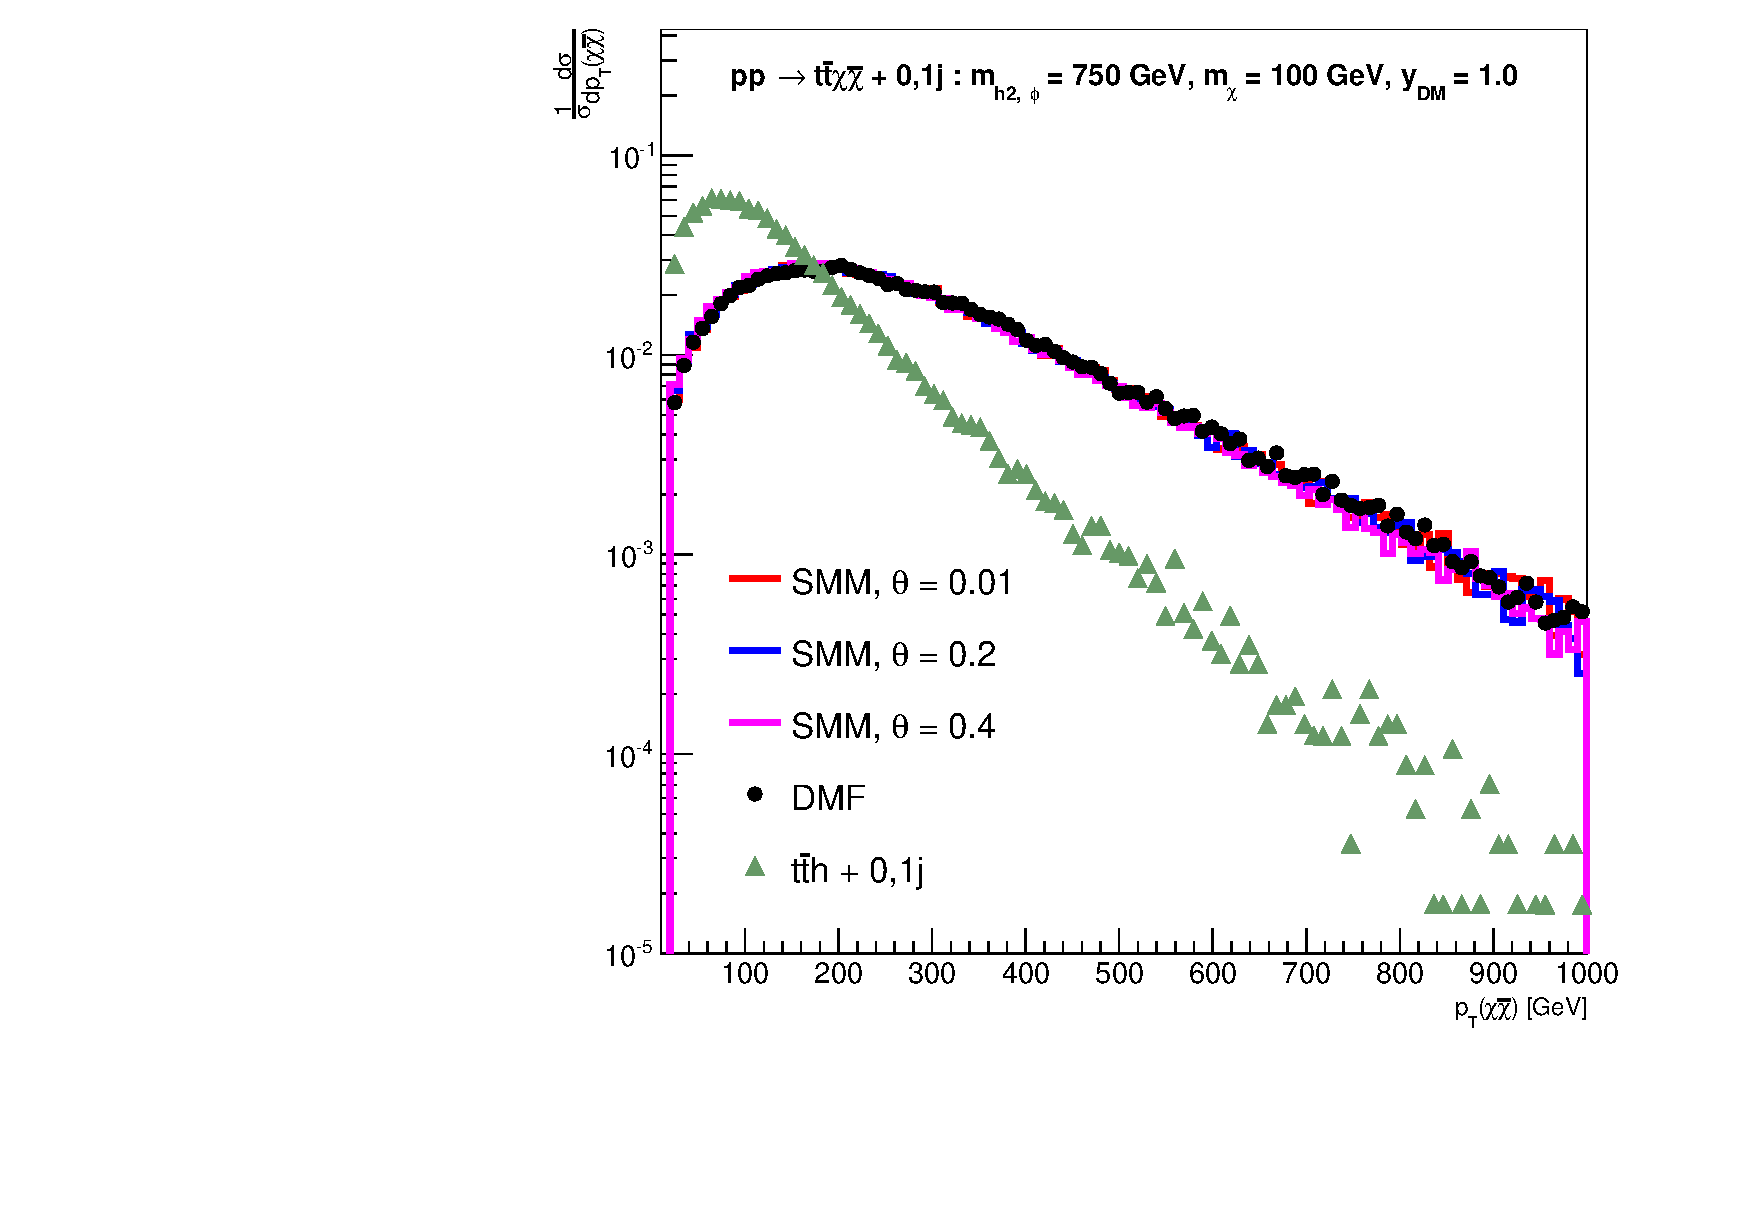
\includegraphics[width=\textwidth]{{./figures/ttDM_kinematics_MMed_750_mDM_100_gDM_1.0_vs_DMF}.pdf}
\end{subfigure}
\begin{subfigure}[b]{0.49\textwidth}
  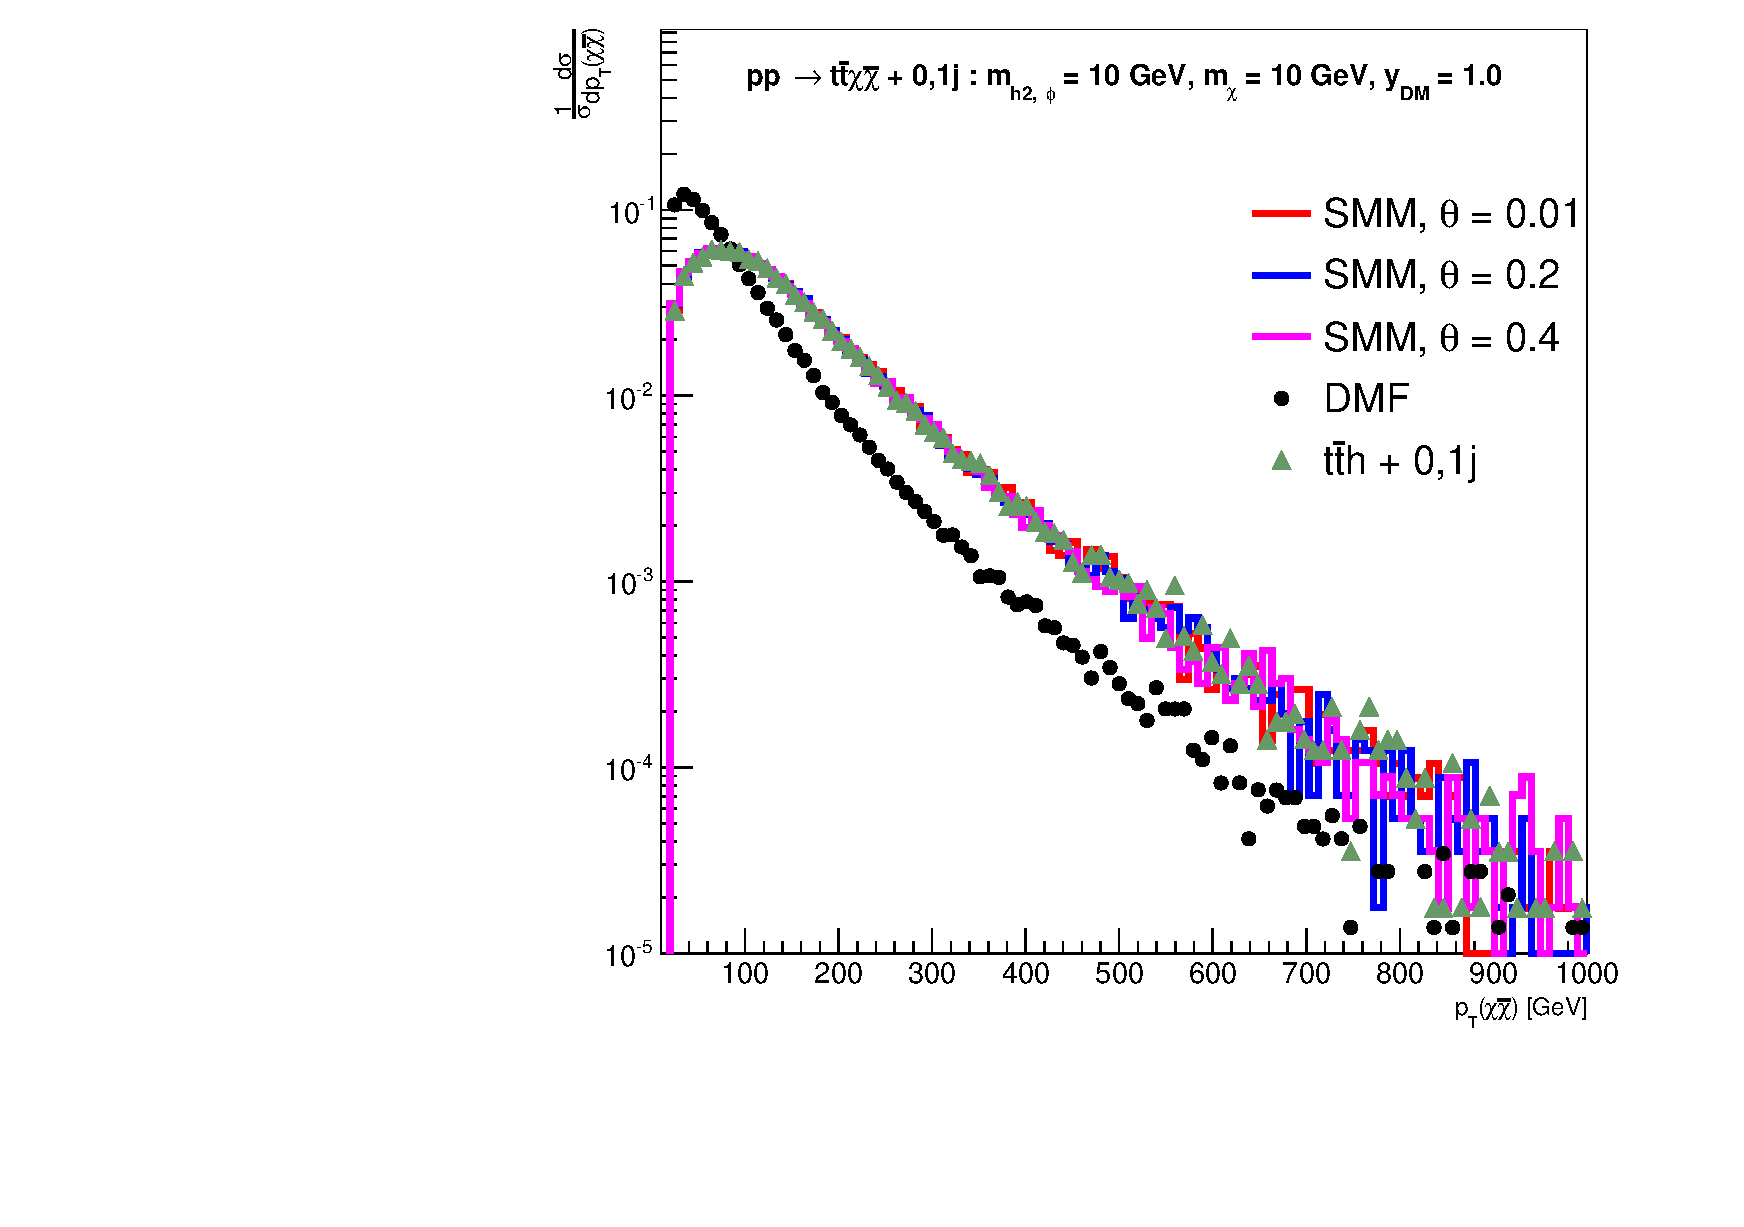
\includegraphics[width=\textwidth]{{./figures/ttDM_kinematics_MMed_10_mDM_10_gDM_1.0_vs_DMF}.pdf}

\end{subfigure}
~\\
  \caption{ Blah ... }
  \label{fig:SMMkinematics}
\end{figure}
%--------------------------------
\begin{figure}[hbtp]
\centering
\begin{subfigure}[b]{0.49\textwidth}
  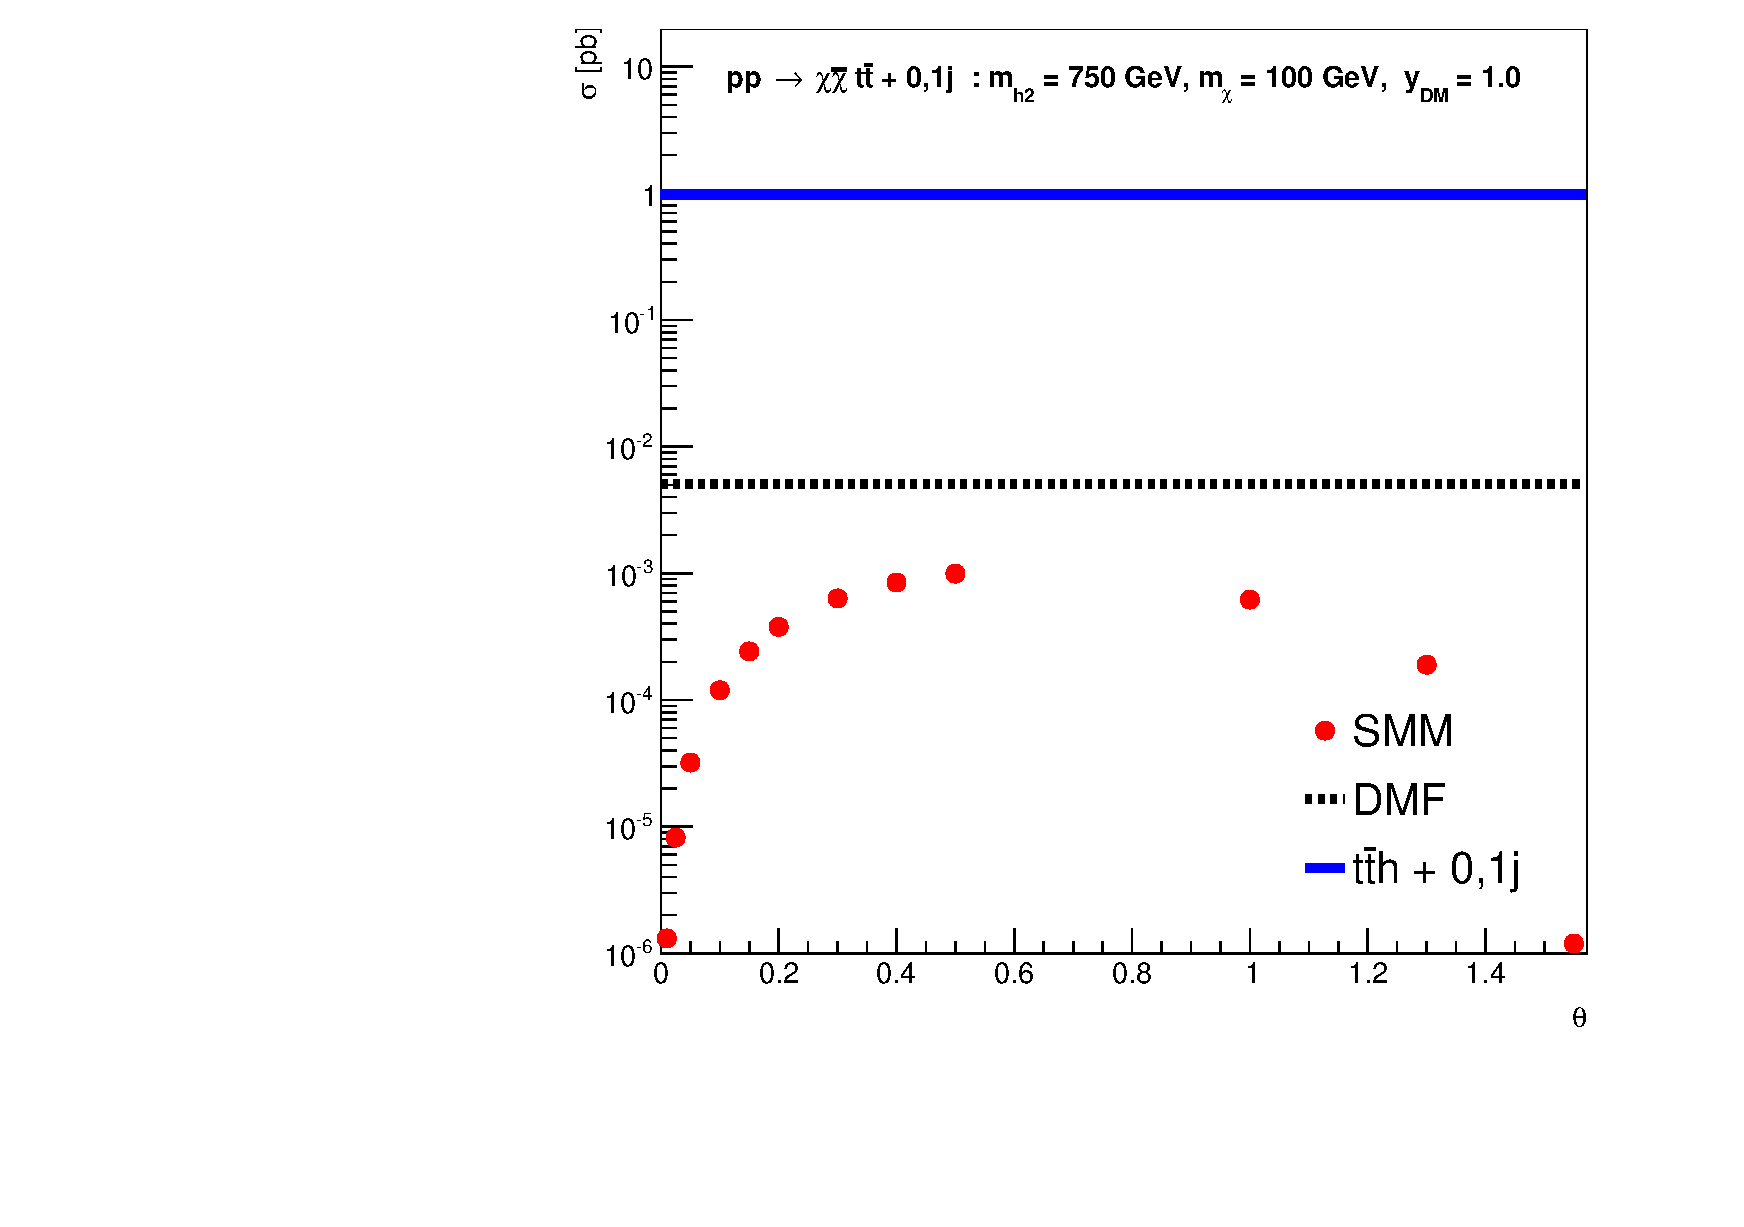
\includegraphics[width=\textwidth]{{./figures/ttDM_xsec_vs_theta_mDM_100_mMed_750_g_1.0}.pdf}
\end{subfigure}
\begin{subfigure}[b]{0.49\textwidth}
  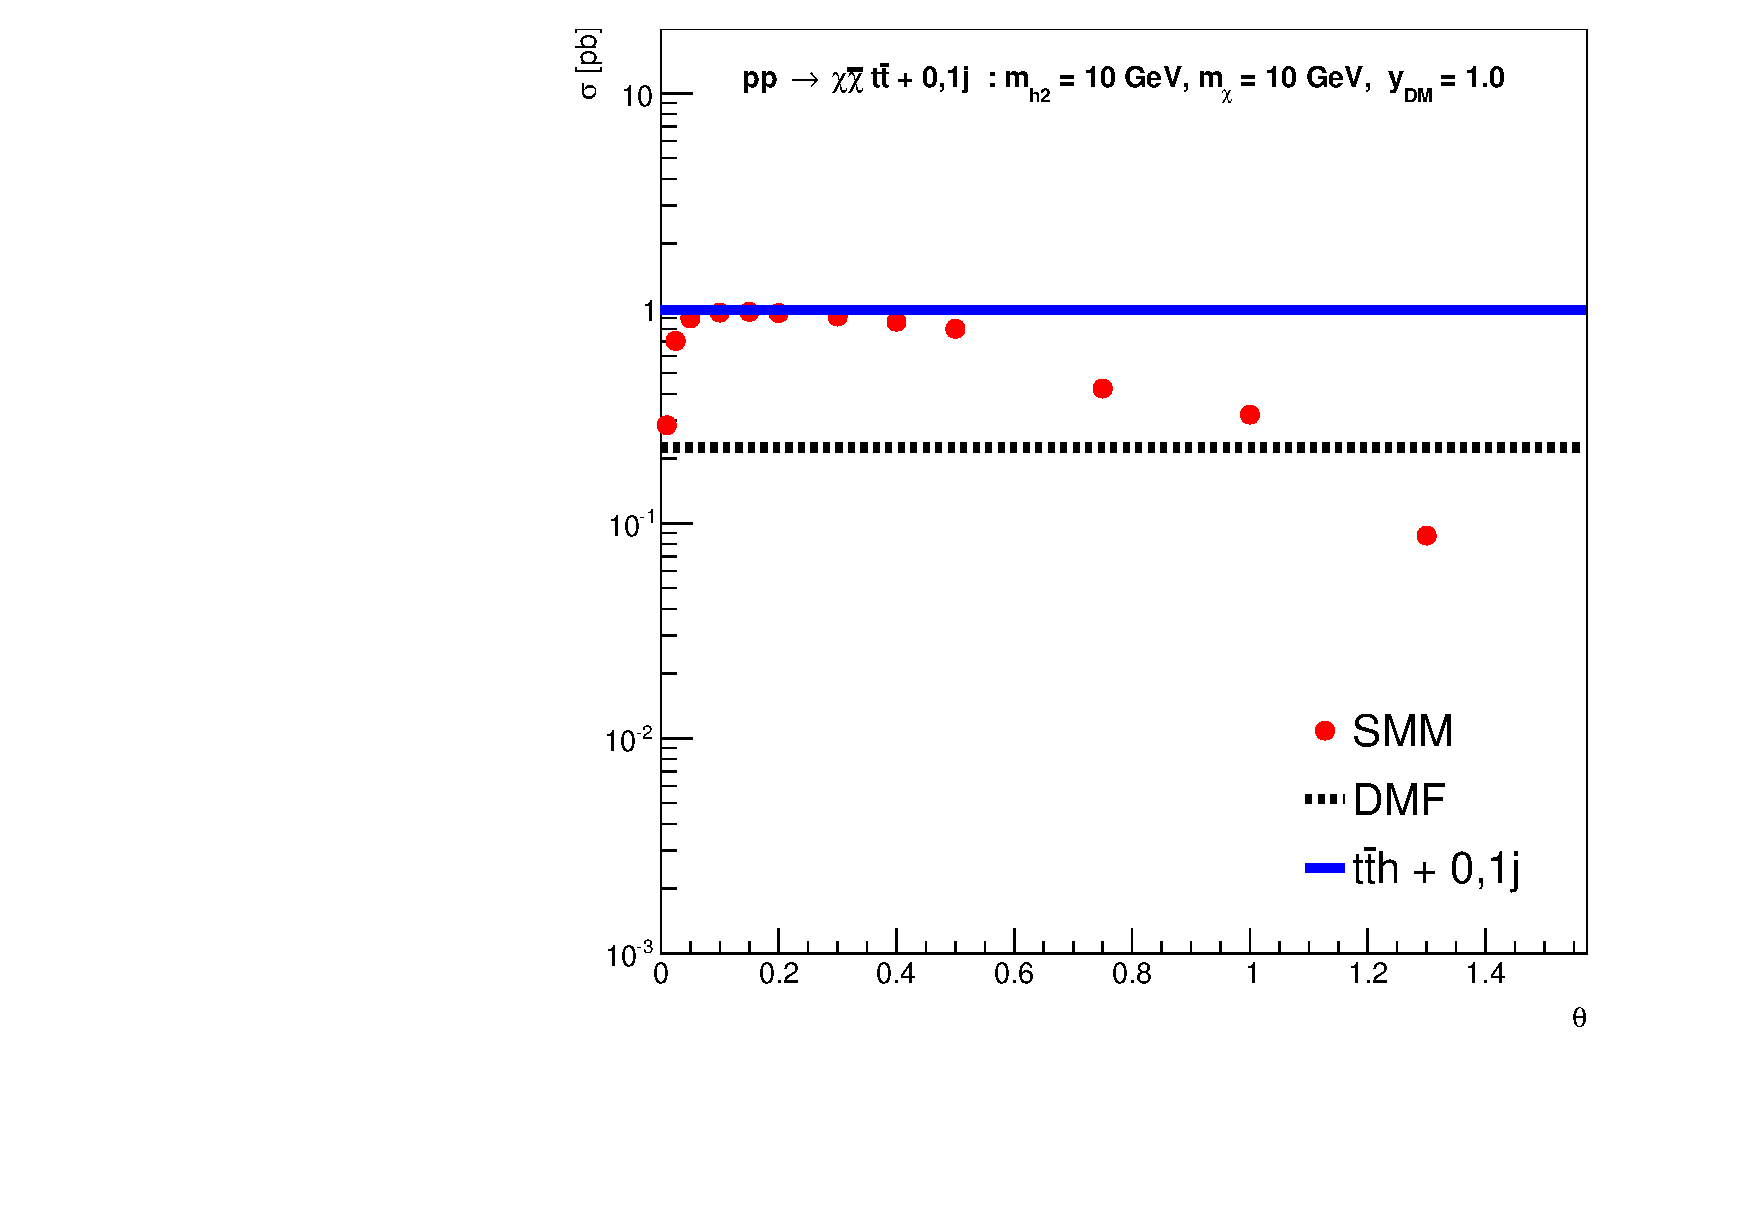
\includegraphics[width=\textwidth]{{./figures/ttDM_xsec_vs_theta_mDM_10_mMed_10_g_1.0}.pdf}
\end{subfigure}
~\\
  \caption{ Blah ... }
  \label{fig:SMMrates}
\end{figure}
%--------------------------------

Mixing between the new scalar and the SM Higgs introduces additional constraints on the SMM relative to the DMF scalar model.  Global fits~\cite{Farzinnia:2013pga,Belanger:2013kya} to LHC Run 1 data find $sin\theta \lesssim 0.4$, which implies that the state h1 (h2) is mostly Higgs-like (singlet-like). Constraints on $\theta$ also arise from the oblique parameters T and S~\cite{Baek:2011aa}, but are weaker than those that follow from the Higgs boson measurements.  LHC searches for invisible Higgs decays can also impose significant constraints on SMM parameters.  For example, Figure~\ref{fig:recast} shows the projected luminosity required to achieve the indicated bounds on $sin\theta$ and $y_{\rm DM}$ from a recasting of the results of Ref.~\cite{CMShinv}.

%--------------------------------
\begin{figure}[hbtp]
\centering
\begin{subfigure}[b]{0.49\textwidth}
  
\includegraphics[width=\textwidth]{./figures/placeholder.jpg}
\end{subfigure}
\begin{subfigure}[b]{0.49\textwidth}
  
\includegraphics[width=\textwidth]{./figures/placeholder.jpg}
\end{subfigure}
~\\
  \caption{ Blah ... }
  \label{fig:recast}
\end{figure}
%--------------------------------

Based on these considerations, we recommend that the following SMM benchmark scenarios be explored: 
~\\
...





%\subsection{Two-Higgs Doublet Models (2HDM)}\label{sub:2hdm} 

%\subsection{t-channel Models}\label{sub:tchannel} 



